\documentclass[border=10pt]{standalone}
\usepackage[svgnames]{xcolor}
\usepackage{amsmath}
\usepackage{pgfplots}
\pgfplotsset{compat=newest}
\usepackage[sfdefault]{FiraSans}
\usepackage{FiraMono}
\renewcommand*\familydefault{\sfdefault}
\begin{document}
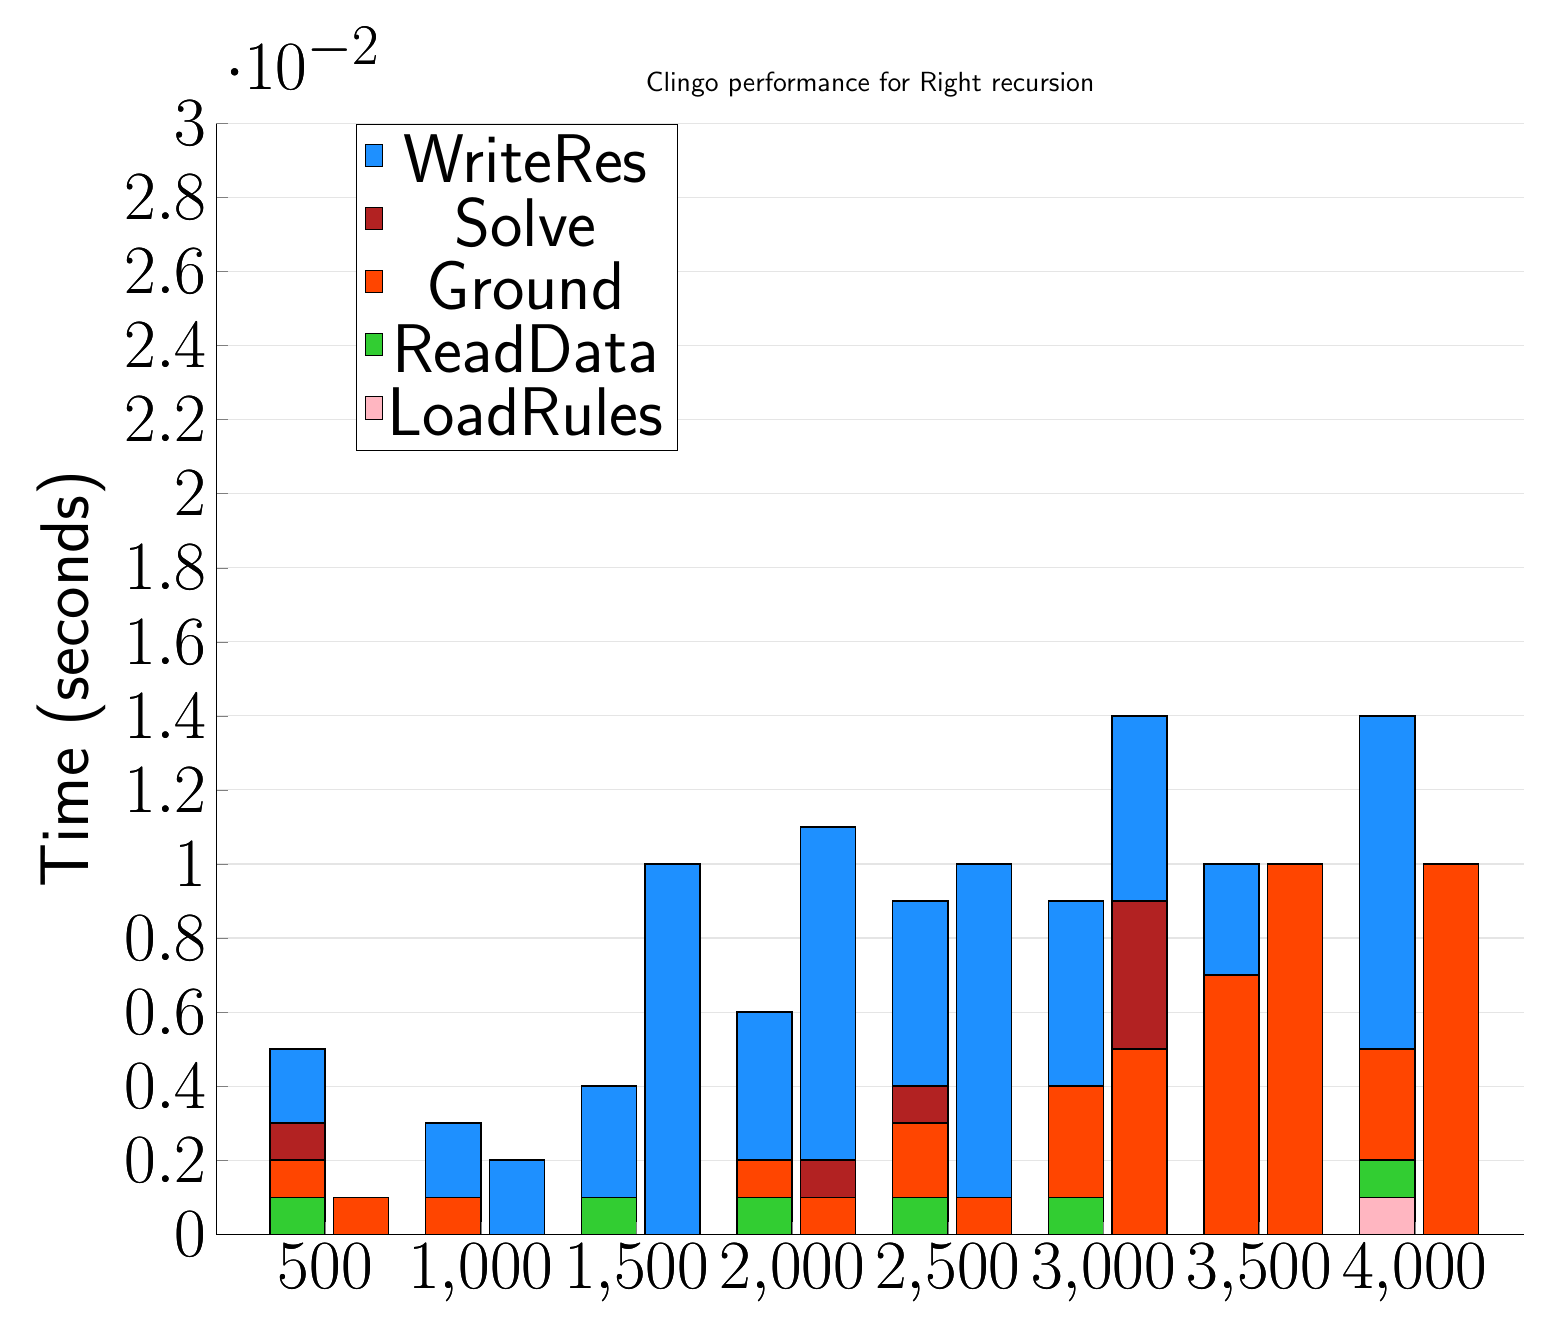
\begin{tikzpicture}
\begin{axis}[
   ybar stacked,
   title={Clingo performance for Right recursion},
   bar shift=-10pt,
   width=1.5\textwidth,
   bar width=0.7cm,
   ymajorgrids, tick align=inside,
   major grid style={draw=gray!20},
   xtick=data,
   ymin=0, ymax=0.029999990463256836,
   axis x line*=bottom,
   axis y line*=left,
   enlarge x limits=0.1,
   legend style={
       at={(0.23, 1)},
       anchor=north,
       legend columns=1,
       font=\Huge,
   },
   ylabel={Time (seconds)},
   label style={font=\Huge},
   tick label style={font=\Huge},
]
\addlegendimage{fill=DodgerBlue, draw=black, line width=0.2pt}
\addlegendentry{WriteRes}
\addlegendimage{fill=FireBrick, draw=black, line width=0.2pt}
\addlegendentry{Solve}
\addlegendimage{fill=OrangeRed, draw=black, line width=0.2pt}
\addlegendentry{Ground}
\addlegendimage{fill=LimeGreen, draw=black, line width=0.2pt}
\addlegendentry{ReadData}
\addlegendimage{fill=LightPink, draw=black, line width=0.2pt}
\addlegendentry{LoadRules}
\addplot +[fill=LightPink, draw=black, line width=0.5pt] coordinates {
    (500, 0.0)
    (1000, 0.0)
    (1500, 0.0)
    (2000, 0.0)
    (2500, 0.0)
    (3000, 0.0)
    (3500, 0.0)
    (4000, 0.0009999990463256836)
};
\addplot +[fill=LimeGreen, draw=black, line width=0.5pt] coordinates {
    (500, 0.0009999990463256836)
    (1000, 0.0)
    (1500, 0.0009999990463256836)
    (2000, 0.0009999990463256836)
    (2500, 0.0009999990463256836)
    (3000, 0.0009999990463256836)
    (3500, 0.0)
    (4000, 0.0009999990463256836)
};
\addplot +[fill=OrangeRed, draw=black, line width=0.5pt] coordinates {
    (500, 0.0009999990463256836)
    (1000, 0.0009999990463256836)
    (1500, 0.0)
    (2000, 0.0009999990463256836)
    (2500, 0.0019999980926513673)
    (3000, 0.0029999971389770507)
    (3500, 0.006999993324279785)
    (4000, 0.0029999971389770507)
};
\addplot +[fill=FireBrick, draw=black, line width=0.5pt] coordinates {
    (500, 0.0009999990463256836)
    (1000, 0.0)
    (1500, 0.0)
    (2000, 0.0)
    (2500, 0.0009999990463256836)
    (3000, 0.0)
    (3500, 0.0)
    (4000, 0.0)
};
\addplot +[fill=DodgerBlue, draw=black, line width=0.5pt] coordinates {
    (500, 0.0019999980926513673)
    (1000, 0.0019999980926513673)
    (1500, 0.0029999971389770507)
    (2000, 0.0039999961853027345)
    (2500, 0.004999995231628418)
    (3000, 0.004999995231628418)
    (3500, 0.0029999971389770507)
    (4000, 0.009000039100646973)
};
\end{axis}
\begin{axis}[
   ybar stacked,
   bar shift=13pt,
   width=1.5\textwidth,
   bar width=0.7cm,
   ymajorgrids, tick align=inside,
   major grid style={draw=none},
   xtick=data,
   ymin=0, ymax=0.029999990463256836,
   axis x line*=none,
   axis y line*=none,
   enlarge x limits=0.1,
   label style={font=\Huge},
   tick label style={font=\Huge},
]
\addplot +[fill=LightPink, draw=black, line width=0.5pt] coordinates {
    (500, 0.0)
    (1000, 0.0)
    (1500, 0.0)
    (2000, 0.0)
    (2500, 0.0)
    (3000, 0.0)
    (3500, 0.0)
    (4000, 0.0)
};
\addplot +[fill=LimeGreen, draw=black, line width=0.5pt] coordinates {
    (500, 0.0)
    (1000, 0.0)
    (1500, 0.0)
    (2000, 0.0)
    (2500, 0.0)
    (3000, 0.0)
    (3500, 0.0)
    (4000, 0.0)
};
\addplot +[fill=OrangeRed, draw=black, line width=0.5pt] coordinates {
    (500, 0.0009999999999999998)
    (1000, 0.0)
    (1500, 0.0)
    (2000, 0.0009999999999999998)
    (2500, 0.0009999999999999998)
    (3000, 0.004999999999999999)
    (3500, 0.009999999999999997)
    (4000, 0.009999999999999997)
};
\addplot +[fill=FireBrick, draw=black, line width=0.5pt] coordinates {
    (500, 0.0)
    (1000, 0.0)
    (1500, 0.0)
    (2000, 0.0009999999999999998)
    (2500, 0.0)
    (3000, 0.003999999999999999)
    (3500, 0.0)
    (4000, 0.0)
};
\addplot +[fill=DodgerBlue, draw=black, line width=0.5pt] coordinates {
    (500, 0.0)
    (1000, 0.0019999999999999996)
    (1500, 0.009999999999999997)
    (2000, 0.008999999999999998)
    (2500, 0.008999999999999998)
    (3000, 0.004999999999999999)
    (3500, 0.0)
    (4000, 0.0)
};
\end{axis}
\end{tikzpicture}

\end{document}
